\documentclass[11pt]{article}
\usepackage{amssymb}
\usepackage{caption}
\usepackage{graphicx}
\usepackage{mathtools}
\usepackage{bookmark}
\graphicspath{ {img/} }
\setlength{\parindent}{0pt}
\DeclareCaptionType{equ}[][]
\usepackage[svgnames]{xcolor}

\usepackage{listings}
\usepackage{color}

\definecolor{dkgreen}{rgb}{0,0.6,0}
\definecolor{gray}{rgb}{0.5,0.5,0.5}
\definecolor{mauve}{rgb}{0.58,0,0.82}

\lstset{frame=tb,
  language=C,
  aboveskip=3mm,
  belowskip=3mm,
  showstringspaces=false,
  columns=flexible,
  basicstyle={\small\ttfamily},
  numbers=none,
  numberstyle=\tiny\color{gray},
  keywordstyle=\color{blue},
  commentstyle=\color{dkgreen},
  stringstyle=\color{mauve},
  breaklines=true,
  breakatwhitespace=true,
  tabsize=3
}

\newcommand*{\plogo}{\fbox{$\mathcal{BM}$}}

\usepackage{PTSerif}

\begin{document} 

\begin{titlepage}

\raggedleft

\vspace*{\baselineskip}

{\Large Bryan Melanson}

\vspace*{0.167\textheight}

\textbf{\LARGE How to Learn}\\[\baselineskip]

{\textcolor{Red}{\Huge Data Structures}}\\[\baselineskip]

{\Large \textit{When your brain doesn't work}}

\vfill

{\large 2021 ~~\plogo}

\vspace*{3\baselineskip}

\end{titlepage}

\pagebreak
%%%%%%%%%%%%%%%%%%%%%%%%%%%%%%%%%%%%%%%%%%%%%%%%%
\pdfbookmark[section]{\contentsname}{toc}
\tableofcontents
\pagebreak
%%%%%%%%%%%%%%%%%%%%%%%%%%%%%%%%%%%%%%%%%%%%%%%%%
\section{Bitwise Operations}
\subsection{Operators}
\begin{list}{}{}
    \item Shift Left \texttt{<<}
    \item Shift Right \texttt{>>}
    \item Or \texttt{|}
    \item And \texttt{\&}
    \item Invert \texttt{\textasciitilde}
    \item Exclusive Or \texttt{\textasciicircum}
\end{list}
\subsection{Common Operations}
In each of the following cases, it should be noted that each byte in hex format is two digits (\texttt{0x00}). Therefore, moving a hex value by one byte is equivalent to shifting it 8 bits, or \texttt{0x00FF << 8 = 0xFF00}, and moving the hex value one space is half a byte, or 4 bits (a \textbf{nibble}). 
\subsubsection{Set Bit}
To set the $n$th bit in value $x$, shift $1$ (\texttt{0x000000001}) by $n$ bits and \texttt{AND} them.
$$\texttt{x \& (1 << n)}$$
\subsubsection{Clear Bit}
To clear the $n$th bit in value $x$, shift $1$ (\texttt{0x000000001}) by $n$ bits and invert the \texttt{AND}ed value.
$$\texttt{x \& \textasciitilde(1 << n)}$$
\subsubsection{Flip Bit}
To flip the $n$th bit in value $x$, shift $1$ (\texttt{0x000000001}) by $n$ bits and \texttt{XOR} them.
$$\texttt{x\textasciicircum  (1 << n)}$$
\subsubsection{Clear}
To clear all values, \texttt{AND} the value with \texttt{0xFFFF}.
$$\texttt{x \&  0xFFFF}$$
\subsubsection{Little Endian to Big Endian}
A little-endian system, in contrast, stores the least-significant byte at the smallest address.

\begin{center}
    \begin{tabular}{ | l | c | c | c | c | c | c | c | c | c | } 
    \hline
    Binary (Decimal: 149) & 1 & 0 & 0 & 1 & 0 & 1 & 0 & 1 \\ 
    \hline
    Bit weight & 2$^7$ & 2$^6$ & 2$^5$ & 2$^4$ & 2$^3$ & 2$^2$ & 2$^1$ & 2$^0$ \\ 
    \hline
    Bit position & MSB & & & & & & & LSB \\ 
    \hline
    \end{tabular}
    \end{center}

In the case of the value \texttt{0x12345678}, the \textbf{least significant byte} of this value \texttt{0x78} is stored in the lowest little Endian address, and subsequent bytes are stored in the next locations. The least significant byte can be considered the byte with the lowest value, when evaluated in typical bitwise fashion: \texttt{0x78563412}

\begin{list}{}{}
    \item \texttt{0x78} \texttt{(0x004000)}
    \item \texttt{0x56} \texttt{(0x004001)}
    \item \texttt{0x34} \texttt{(0x004002)}
    \item \texttt{0x12} \texttt{(0x004003)}
\end{list}

\subsubsection{Big Endian to Little Endian}

In a Big Endian representation of \texttt{0x12345678}, the \textbf{most significant byte} (\texttt{0x12}) is stored at the lowest memory address: \texttt{0x12345678}

\begin{list}{}{}
    \item \texttt{0x12} \texttt{(0x004000)}
    \item \texttt{0x34} \texttt{(0x004001)}
    \item \texttt{0x56} \texttt{(0x004002)}
    \item \texttt{0x78} \texttt{(0x004003)}
\end{list}

To reverse these positions, the bytes can be isolated and bit-shifted by the appropriate number of bits to form the appropriate order.

\begin{list}{}{}
\item \texttt{(0x12345678 \& 0x000000FF) << 24}
\item \texttt{(0x12345678 \& 0x0000FF00) << 16}
\item \texttt{(0x12345678 \& 0x00FF0000) << 8}
\item \texttt{(0x12345678 \& 0xFF000000) >> 24}
\end{list}

%%%%%%%%%%%%%%%%%%%%%%%%%%%%%%%%%%%%%%%%%%%%%%%%%
\section{Array}
Arrays are collections of same-type data items stored in a contiguous memory location. Knowing the data type, each element is located at an offset based on that data size. In other words, for \texttt{int data[]} the data at \texttt{data[1]} is located at \texttt{data[0] + sizeof(int)}.
\begin{center}
    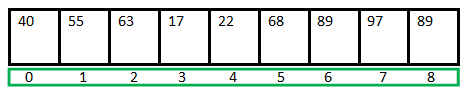
\includegraphics[width=250 px]{img/array}  \\
\end{center}
\subsection{Arrays in C}
There is no index out-of-bound checking in C, so if access goes beyond the index boundaries of the array (\texttt{0-(n-1)}) there will be undefined behavior.
\subsection{Static vs. Dynamic Arrays}
Pointer and array accesses can be treated the same way in C, either by accessing the values by using the [] operator, or by incrementing the value of the pointer. 
\subsubsection{Static Arrays}
In C, the size of an array should be decided at compile time by defining the array size either by declaring an array with size constraints such as \texttt{arr[10]} or by using \texttt{malloc} to define the required size. At run time this size will be used to allocate the required memory space.
\subsubsection{Dynamic Arrays}
In C++ an array can be passed a variable and the size can be determined for the memory allocation at run time.
\subsection{C Strings}
A C string is a pointer to an array of \texttt{char} data items which is terminated by the \texttt{NULL} character at the size limit. So, a \texttt{char} array of \texttt{n} items will contain data at elements \texttt{0-(n-1)}, while the value at \texttt{n} will be \texttt{NULL}. This allows for string operations to check for the boundary of memory space for the string object.
%%%%%%%%%%%%%%%%%%%%%%%%%%%%%%%%%%%%%%%%%%%%%%%%%
\section{Matrix}
\begin{center}
    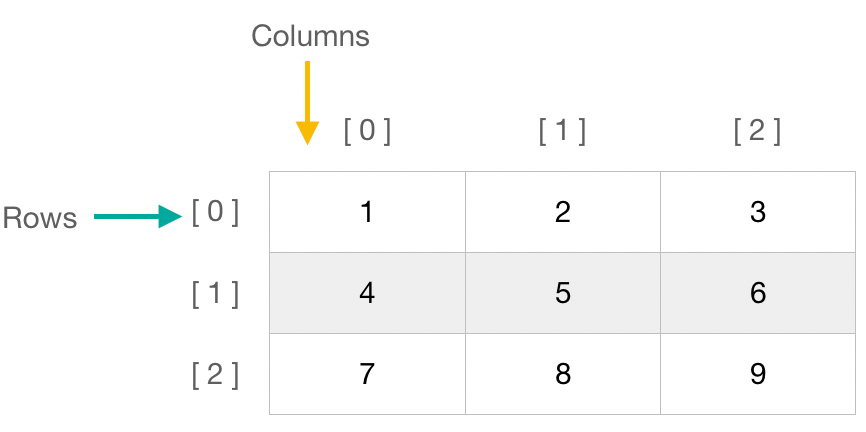
\includegraphics[width=250 px]{img/matrix}  \\
\end{center}
\subsection{Normal Declaration}
\subsection{Dynamic Declaration}
%%%%%%%%%%%%%%%%%%%%%%%%%%%%%%%%%%%%%%%%%%%%%%%%%
\section{Linked List}
Unlike arrays, Linked Lists are dynamic and can grow by pointing to non-contiguous locations in memory using pointers. Extra memory is required when representing each pointer in the linked list, but it allows for easily inserting and deleting objects in the linekd list.
\begin{center}
    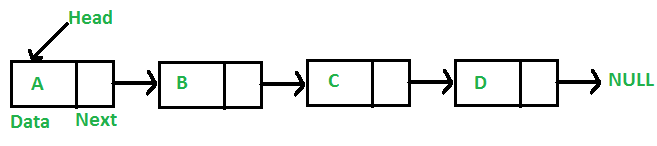
\includegraphics[width=250 px]{img/linkedlist}  \\
\end{center}
Each node in the linked list consists of its data, and a pointer to the next object in the linked list. In the case that the head of the linked list is null.


\subsection{Inserting}



\subsection{Deleting}



\section{Circular Linked List}



\subsection{Inserting}



\subsection{Deleting}

\begin{center}
    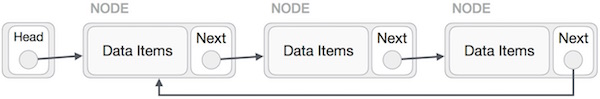
\includegraphics[width=350 px]{img/circularlinkedlist}  \\
\end{center}
\section{Doubly Linked List}
\begin{center}
    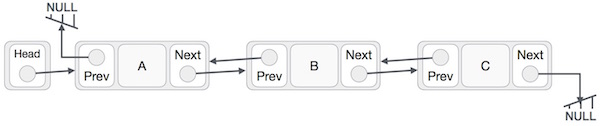
\includegraphics[width=350 px]{img/doublylinkedlist}  \\
\end{center}



\subsection{Inserting}



\subsection{Deleting}



%%%%%%%%%%%%%%%%%%%%%%%%%%%%%%%%%%%%%%%%%%%%%%%%%
\section{Binary Tree}
\begin{center}
    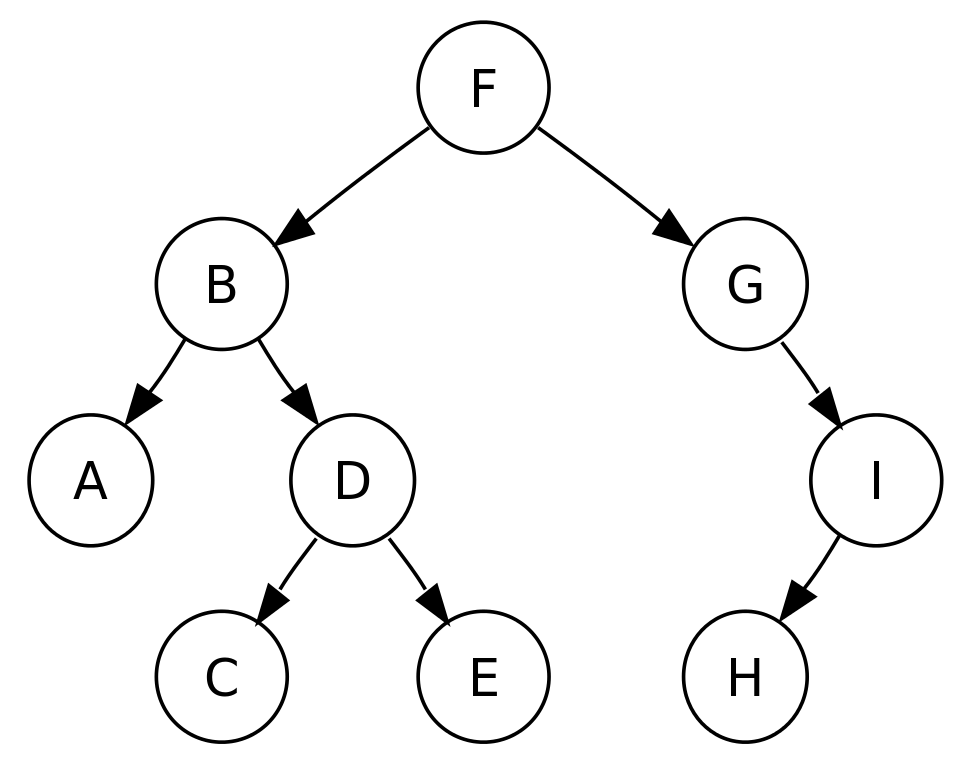
\includegraphics[width=250 px]{img/binarytree}  \\
\end{center}

A Binary Tree is any tree organized in which each node, or \textbf{root} has at most two children, or \textbf{leaves}, hence \textit{binary}, designated left and right. 

\subsection{Depth First Traversal}

\textbf{Depth First Traversal} traverses the tree to its extents before backtracking and completing the traversal. It will explore until it reaches nodes with no children before moving to the nearest neighbor. The order of traversal can be categorized into \textbf{Pre-Order}, \textbf{In-Order} and \textbf{Post-Order} which determine which order the nodes (\textit{Left},\textit{right},\textit{center}) are visited.

\subsubsection{Pre-Order Traversal}
\begin{lstlisting}
void pre_order(struct Node* n) {
    // print n->value

    if (n->left)
        pre_order(n->left);

    if (n->right)
        pre_order(n->right);
}
\end{lstlisting}
\subsubsection{In-Order Traversal}
\begin{lstlisting}
void in_order(struct Node* n) {
    if (n->left)
        pre_order(n->left);

    // print n->value

    if (n->right)
        pre_order(n->right);
}
\end{lstlisting}
\subsubsection{Post-Order Traversal}
\begin{lstlisting}
void post_order(struct Node* n) {
    if (n->left)
        pre_order(n->left);

    if (n->right)
        pre_order(n->right);

    // print n->value
}
\end{lstlisting}
\subsection{Breadth First Traversal}

Breadth first traversal traverses a tree by visiting all nodes at a given height, before descending the depth of the tree.

\begin{lstlisting}
def bfs(self):
    queue = Queue()
    queue.put(self)

    while not queue.empty():
        current_node = queue.get()
        print(current_node.value)

        if current_node.left_child:
            queue.put(current_node.left_child)

        if current_node.right_child:
            queue.put(current_node.right_child)
\end{lstlisting}

%%%%%%%%%%%%%%%%%%%%%%%%%%%%%%%%%%%%%%%%%%%%%%%%%
\section{AVL Tree}
%%%%%%%%%%%%%%%%%%%%%%%%%%%%%%%%%%%%%%%%%%%%%%%%%
\section{Red-Black Tree}
%%%%%%%%%%%%%%%%%%%%%%%%%%%%%%%%%%%%%%%%%%%%%%%%%
\section{N-Ary Tree}
%%%%%%%%%%%%%%%%%%%%%%%%%%%%%%%%%%%%%%%%%%%%%%%%%
\section{Binary Search Tree}
\begin{center}
    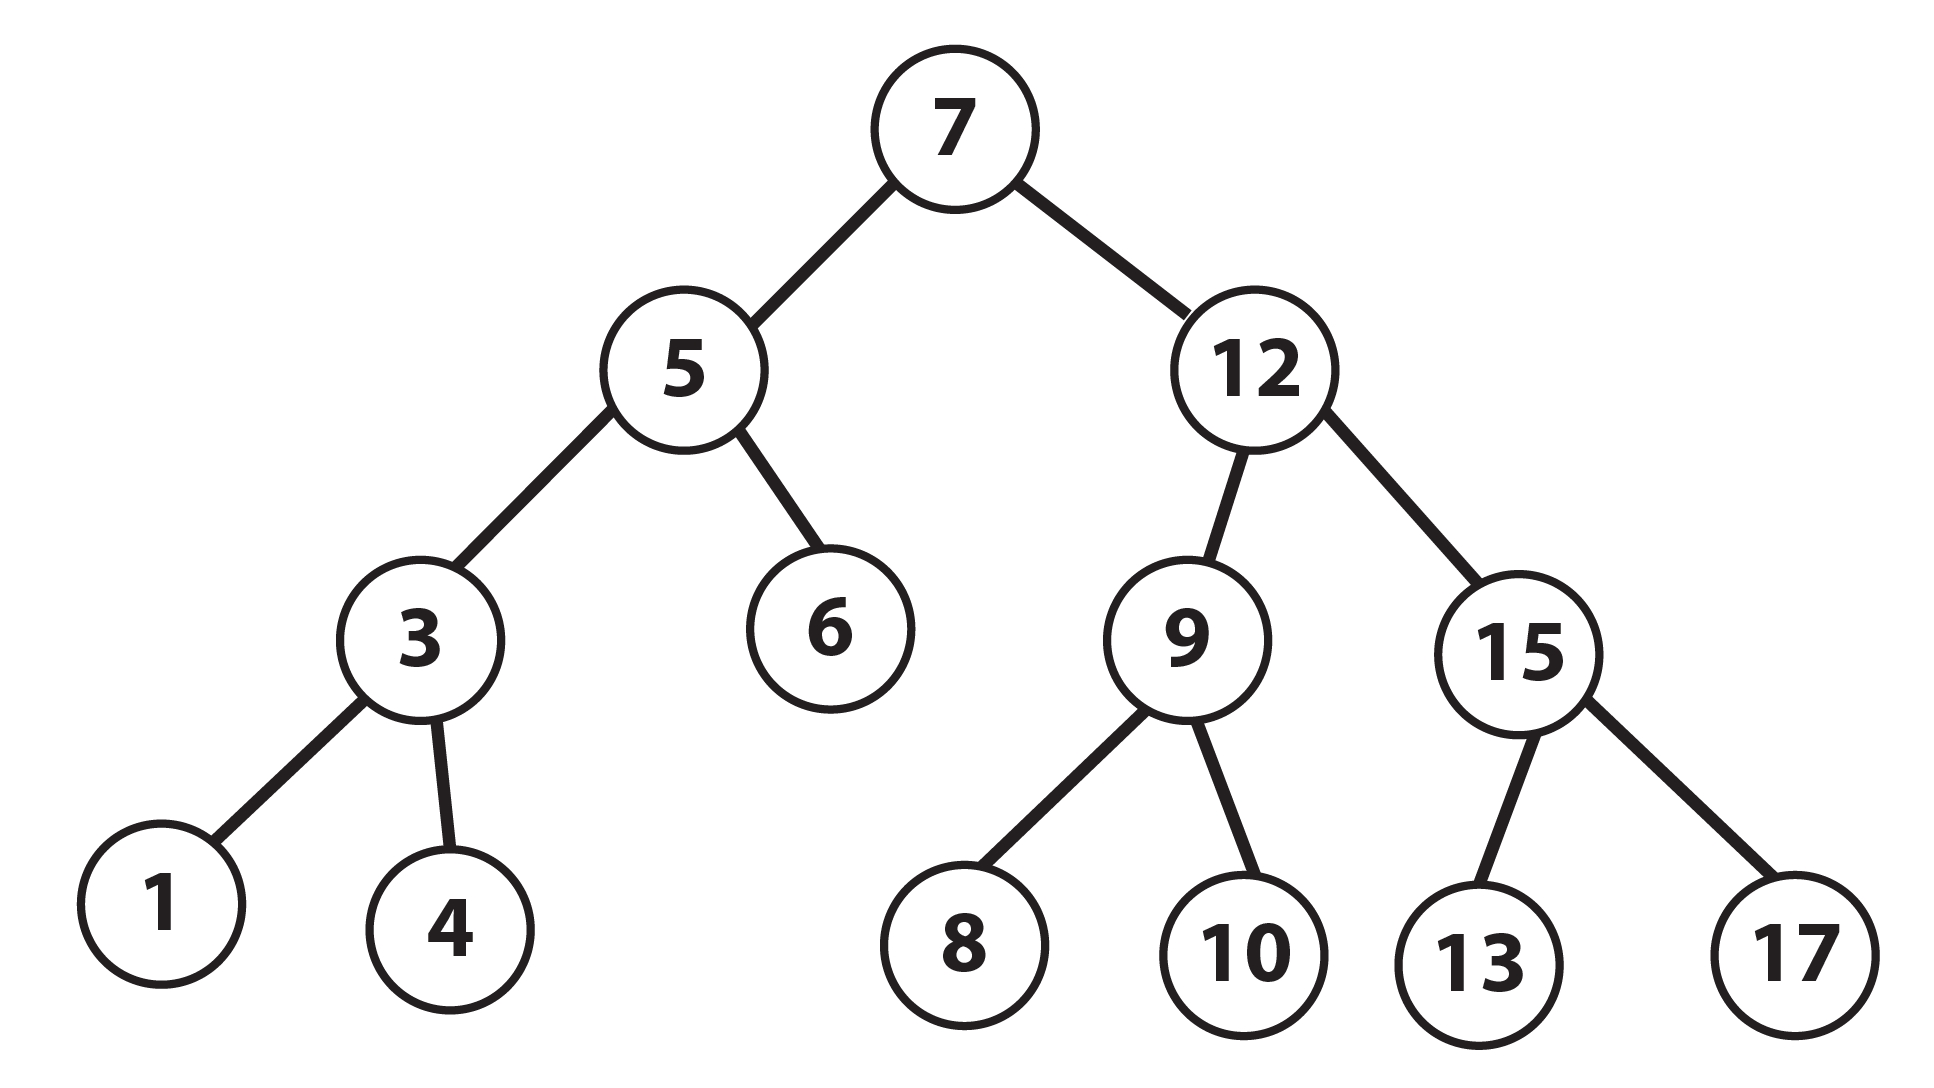
\includegraphics[width=250 px]{img/binarysearchtree}  \\
\end{center}

A Binary Search Tree is one in which the value of the node stored on the left is less than the value of root, and the value of the node on the right is greater than the value of the root. By organizing a tree in this way, values can easily be found using a similar method as binary search which eliminates half of the remaining possibilities at each step.

\subsection{Searching}

\begin{lstlisting}
bool contains(Node* curr, int value) {
    if (curr->data == value) { return true; }
    else if (value < curr->value) {
        if (curr->left) {
            return contains(curr->left, value);
        }
    } else {
        if (curr->right) {
            return contains(curr->right, value);
        }
    }
}
\end{lstlisting}

\subsection{Inserting}

To maintain the structure rules of the Binary Search Tree after insertion, the leaves of each node must be evaluated and the next route determined until a non-null spot that meets the criteria is determined. If the the current value of the node is greater than the value to be inserted, it will attempt to insert on the left if the left is currently null. If the left is not null, it will recursively evaluate the left node in the same way.

\begin{lstlisting}
void insert(Node* new, Node* curr, int value) {
    if (value <= curr->value) {
        if (curr->left == NULL) {
            curr->left = new;
        } else {
            insert(curr->left, value);
        }
    } else {
        if (curr->right == NULL) {
            curr->right = new;
        } else {
            insert(curr->right, value);
        }
    }
}
\end{lstlisting}

%%%%%%%%%%%%%%%%%%%%%%%%%%%%%%%%%%%%%%%%%%%%%%%%%
\section{B-Tree}

%%%%%%%%%%%%%%%%%%%%%%%%%%%%%%%%%%%%%%%%%%%%%%%%%
\section{Stack}
\begin{center}
    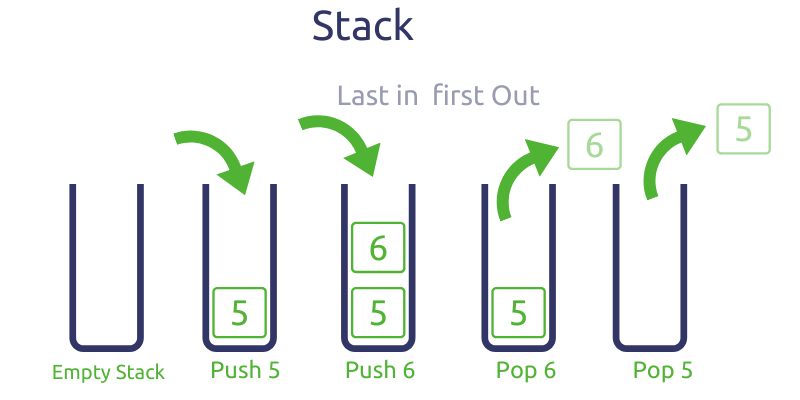
\includegraphics[width=250 px]{img/stack}  \\
\end{center}

\subsection{Stack Array}

A struct can be created which tracks the index of the top, and holds the allocated array. When popping a value, the array index should be wiped with a \texttt{null} value and top decremented. If the top index is out of range, it should throw an error to indicate a stack underflow.

\begin{lstlisting}
/*
* Stack implementation using array in C
*/

#define CAPACITY 100

typedef struct stack {
    int top;
    arr[CAPACITY];
} stack;

// Function to push a new element in stack
void push(stack* s, int val)
{
    s->arr[s->top++] = val;
}

// Function to pop element from top of stack
int pop(stack* s)
{    
    if (top < 0) return -1;
    return s->arr[s->top--];
}
\end{lstlisting}

\subsection{Dynamic Stack Using Linked List}

When the size of the array is not known and allocating a static array of its capacity may be wasteful, Linked Lists can be used to connect the items on the stack. When popping an object, the node pointer should be stored in a temporary pointer, then free'd once the new top is the old node's next pointer.

\begin{lstlisting}
/*
* Stack implementation using linked list in C
*/

// Define stack node structure
// The variable also instantiates this as a global
struct stack {
    int data;
    struct stack *next;
} *top;

// Function to push a new element in stack.
void push(int element)
{
    // Create a new node and push to stack
    struct stack* newNode = malloc(sizeof(struct stack));

    // Assign data to new node in stack
    newNode->data = element;

    // Next element after new node should be current top element
    newNode->next = top;        

    // Make sure new node is always at top
    top = newNode;
}

// Function to pop element from top of stack.
int pop()
{    
    // Check stack underflow
    if (!top)
    {
        printf("Stack is empty.\n");
        return -1;
    }
    // Hold pointer to node to be removed
    stack* old = top;
    
    int data = 0;
 
    // Copy data from stack's top element
    data = old->data;

    // Move top to its next element
    top = old->next;

    free(old);

    return data;
}
\end{lstlisting}
%%%%%%%%%%%%%%%%%%%%%%%%%%%%%%%%%%%%%%%%%%%%%%%%%
\section{Queue}
\begin{center}
    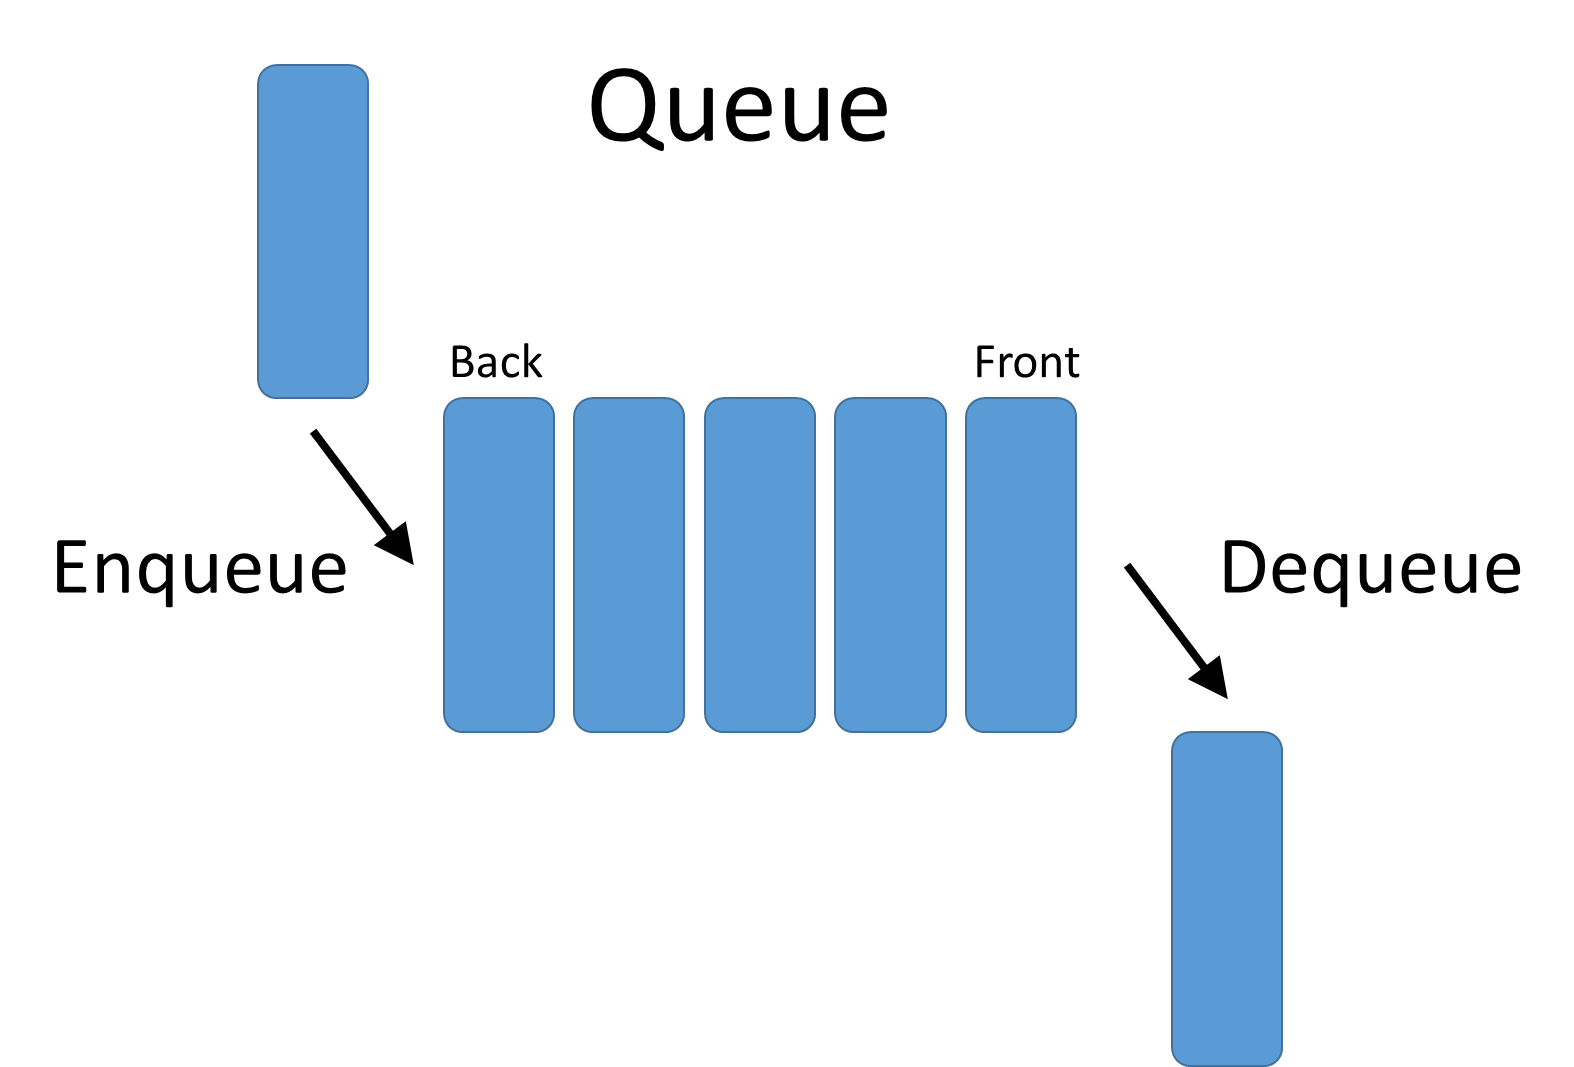
\includegraphics[width=200 px]{img/queue}  \\
\end{center}
%%%%%%%%%%%%%%%%%%%%%%%%%%%%%%%%%%%%%%%%%%%%%%%%%
\section{Heap}
\begin{center}
    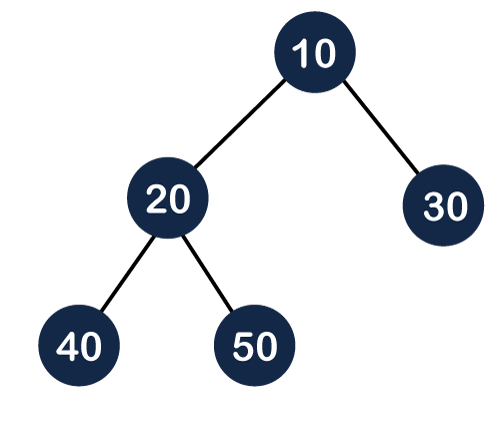
\includegraphics[width=200 px]{img/heap}  \\
\end{center}
\subsection{Maximimum Heap}
\subsection{Minimum Heap}
%%%%%%%%%%%%%%%%%%%%%%%%%%%%%%%%%%%%%%%%%%%%%%%%%
\section{Hashes}
\begin{center}
    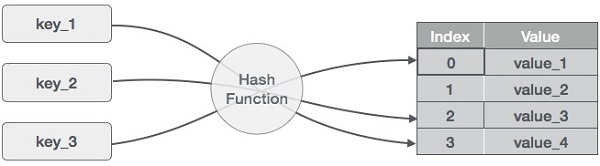
\includegraphics[width=300 px]{img/hash}  \\
\end{center}

A hash map combines features of a static array and a linked list, without being bound by issues such as inserting new values in a size-defined array, or searching for values in a linked list. A hash map has a preallocated buffer, and uses the value of the data to be inserted to generate a key, or index by hashing it. If a hash is properly defined, there will be no hash collisions, and data with an indentical value will be stored in the identical spot in the hash map. This way, a value need only be calculated once, then stored in the hash map. Insted of generating the value again by calculation, the value can be retrieved from the hash map by visiting the pre-determined index.
\\
\\
The \textbf{Hash Set} is a hash map which stores no repeated values.

\subsection{Code}
\begin{lstlisting}
int hash(int key) {
    int r = key % SIZE;
    return r < 0 ? r + SIZE : r;
}

void insert(int *values, int key, int value) {
    int index = hash(key);
    while (values[index]) {
        index++;
        index %= SIZE;
    }
    keys[index] = key;
    values[index]= value;
}

int search(int *keys, int *values, int key) {
    int index = hash(key);
    while (values[index]) {
        if (keys[index] == key) {
            return values[index];
        }
        index++;
        index %= SIZE;
    }
    return 0;
}

/* The requested value is checked for, in each step of the loop then the hash map is populated with the value if it doesn't already exist. This means the check will take O(n) */

int* main(int* nums, int numsSize, int target) {
    int keys[SIZE];
    int values[SIZE] = {0};
    for (int i = 0; i < numsSize; i++) {
        int complements = target - nums[i];
        int value = search(keys, values, complements);
        if (value) {
            int *indices = (int *) malloc(sizeof(int) * 2);
            indices[0] = value - 1;
            indices[1] = i;
            return indices;
        }
        insert(keys, values, nums[i], i + 1);
    }
    return NULL;
}
\end{lstlisting}

\subsection{Hash Functions}

\begin{table}
    
\end{table}

\subsubsection{Simple Hash Function for Strings}
\begin{lstlisting}
    int hash_function(char* key) {
        int hash = toupper(key[0]) - 'A'; 
        /* Subtracting 'A' sets the index of alpha characters starting with 0 for 'A'. 'A' is 0, 'B' is 1, etc. */
        return hash % SIZE; // Constrain to the array size
    }
\end{lstlisting}

If a collision occurs, linked lists can point to values with this same index.

A good hash value would distribute values evenly across the map.

%%%%%%%%%%%%%%%%%%%%%%%%%%%%%%%%%%%%%%%%%%%%%%%%%
\section{Graph}
\begin{center}
    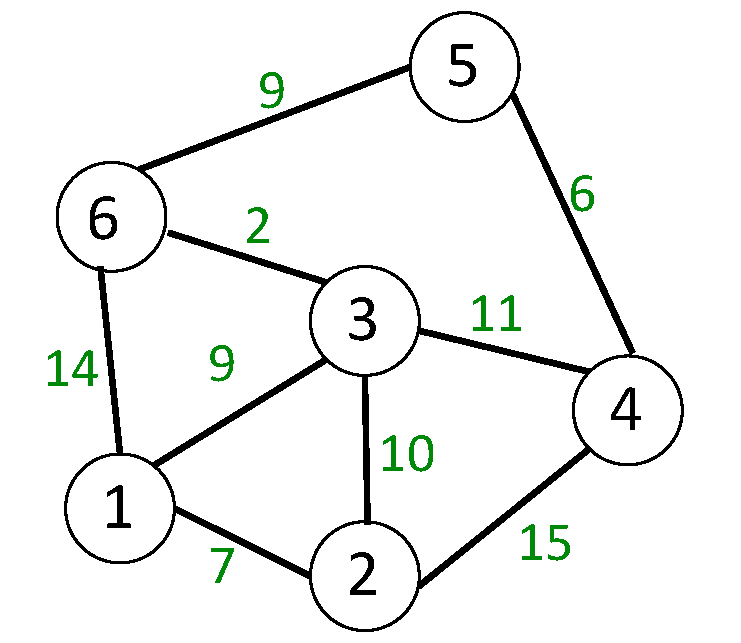
\includegraphics[width=200 px]{img/graph}  \\
\end{center}
%%%%%%%%%%%%%%%%%%%%%%%%%%%%%%%%%%%%%%%%%%%%%%%%%
\end{document}
